%\VignetteIndexEntry{Introduction to the USGSHydroOpt package}
%\VignetteEngine{knitr::knitr}
%\VignetteDepends{}
%\VignetteSuggests{}
%\VignetteImports{reshape2}
%\VignettePackage{USGSHydroOpt}

\documentclass[a4paper,11pt]{article}\usepackage[]{graphicx}\usepackage[]{color}
%% maxwidth is the original width if it is less than linewidth
%% otherwise use linewidth (to make sure the graphics do not exceed the margin)
\makeatletter
\def\maxwidth{ %
  \ifdim\Gin@nat@width>\linewidth
    \linewidth
  \else
    \Gin@nat@width
  \fi
}
\makeatother

\definecolor{fgcolor}{rgb}{0.345, 0.345, 0.345}
\newcommand{\hlnum}[1]{\textcolor[rgb]{0.686,0.059,0.569}{#1}}%
\newcommand{\hlstr}[1]{\textcolor[rgb]{0.192,0.494,0.8}{#1}}%
\newcommand{\hlcom}[1]{\textcolor[rgb]{0.678,0.584,0.686}{\textit{#1}}}%
\newcommand{\hlopt}[1]{\textcolor[rgb]{0,0,0}{#1}}%
\newcommand{\hlstd}[1]{\textcolor[rgb]{0.345,0.345,0.345}{#1}}%
\newcommand{\hlkwa}[1]{\textcolor[rgb]{0.161,0.373,0.58}{\textbf{#1}}}%
\newcommand{\hlkwb}[1]{\textcolor[rgb]{0.69,0.353,0.396}{#1}}%
\newcommand{\hlkwc}[1]{\textcolor[rgb]{0.333,0.667,0.333}{#1}}%
\newcommand{\hlkwd}[1]{\textcolor[rgb]{0.737,0.353,0.396}{\textbf{#1}}}%

\usepackage{framed}
\makeatletter
\newenvironment{kframe}{%
 \def\at@end@of@kframe{}%
 \ifinner\ifhmode%
  \def\at@end@of@kframe{\end{minipage}}%
  \begin{minipage}{\columnwidth}%
 \fi\fi%
 \def\FrameCommand##1{\hskip\@totalleftmargin \hskip-\fboxsep
 \colorbox{shadecolor}{##1}\hskip-\fboxsep
     % There is no \\@totalrightmargin, so:
     \hskip-\linewidth \hskip-\@totalleftmargin \hskip\columnwidth}%
 \MakeFramed {\advance\hsize-\width
   \@totalleftmargin\z@ \linewidth\hsize
   \@setminipage}}%
 {\par\unskip\endMakeFramed%
 \at@end@of@kframe}
\makeatother

\definecolor{shadecolor}{rgb}{.97, .97, .97}
\definecolor{messagecolor}{rgb}{0, 0, 0}
\definecolor{warningcolor}{rgb}{1, 0, 1}
\definecolor{errorcolor}{rgb}{1, 0, 0}
\newenvironment{knitrout}{}{} % an empty environment to be redefined in TeX

\usepackage{alltt}
\usepackage{amsmath}
\usepackage{times}
\usepackage{hyperref}
\usepackage[numbers, round]{natbib}
\usepackage[american]{babel}
\usepackage{authblk}
\usepackage{subfig}
\usepackage{placeins}
\usepackage{footnote}
\usepackage{tabularx}
\usepackage{parskip}
\usepackage{threeparttable}
\renewcommand\Affilfont{\itshape\small}

\renewcommand{\topfraction}{0.85}
\renewcommand{\textfraction}{0.1}
\usepackage{graphicx}

\textwidth=6.5in
\textheight=9.2in
\parskip=.3cm
\oddsidemargin=.1in
\evensidemargin=.1in
\headheight=-.3in

%------------------------------------------------------------
% newcommand
%------------------------------------------------------------
\newcommand{\scscst}{\scriptscriptstyle}
\newcommand{\scst}{\scriptstyle}
\newcommand{\Robject}[1]{{\texttt{#1}}}
\newcommand{\Rfunction}[1]{{\texttt{#1}}}
\newcommand{\Rclass}[1]{\textit{#1}}
\newcommand{\Rpackage}[1]{\textit{#1}}
\newcommand{\Rexpression}[1]{\texttt{#1}}
\newcommand{\Rmethod}[1]{{\texttt{#1}}}
\newcommand{\Rfunarg}[1]{{\texttt{#1}}}
\IfFileExists{upquote.sty}{\usepackage{upquote}}{}
\begin{document}






%------------------------------------------------------------
\title{Introduction to USGSHydroOpt}
%------------------------------------------------------------
\author[1]{Samuel Christel}
\author[1]{Steve Corsi}
\affil[1]{United States Geological Survey}




\maketitle
\tableofcontents

%------------------------------------------------------------
\section{Introduction to USGSHydroOpt}
%------------------------------------------------------------ 
The USGSHydroOpt package was created to streamline the process of creating optical summary variables and excitation-emission (EEMs) plots for absorbance and fluoresence data collected from various freshwater sources. Examples of optical summary variables that can be produced with this package include various absorbance peaks, The functions in this package were designed to operate on dataframes with a standardized structures. This package is not amenable to dataframes that do not fit the prescribed format. The example dataframes in this package illustrate exactly how dataframes should be formatted, and the examples illustrate how the functions operate on the dataframes. Depicted below is an example of an EEMs plot produced with this package.

\begin{knitrout}
\definecolor{shadecolor}{rgb}{0.969, 0.969, 0.969}\color{fgcolor}
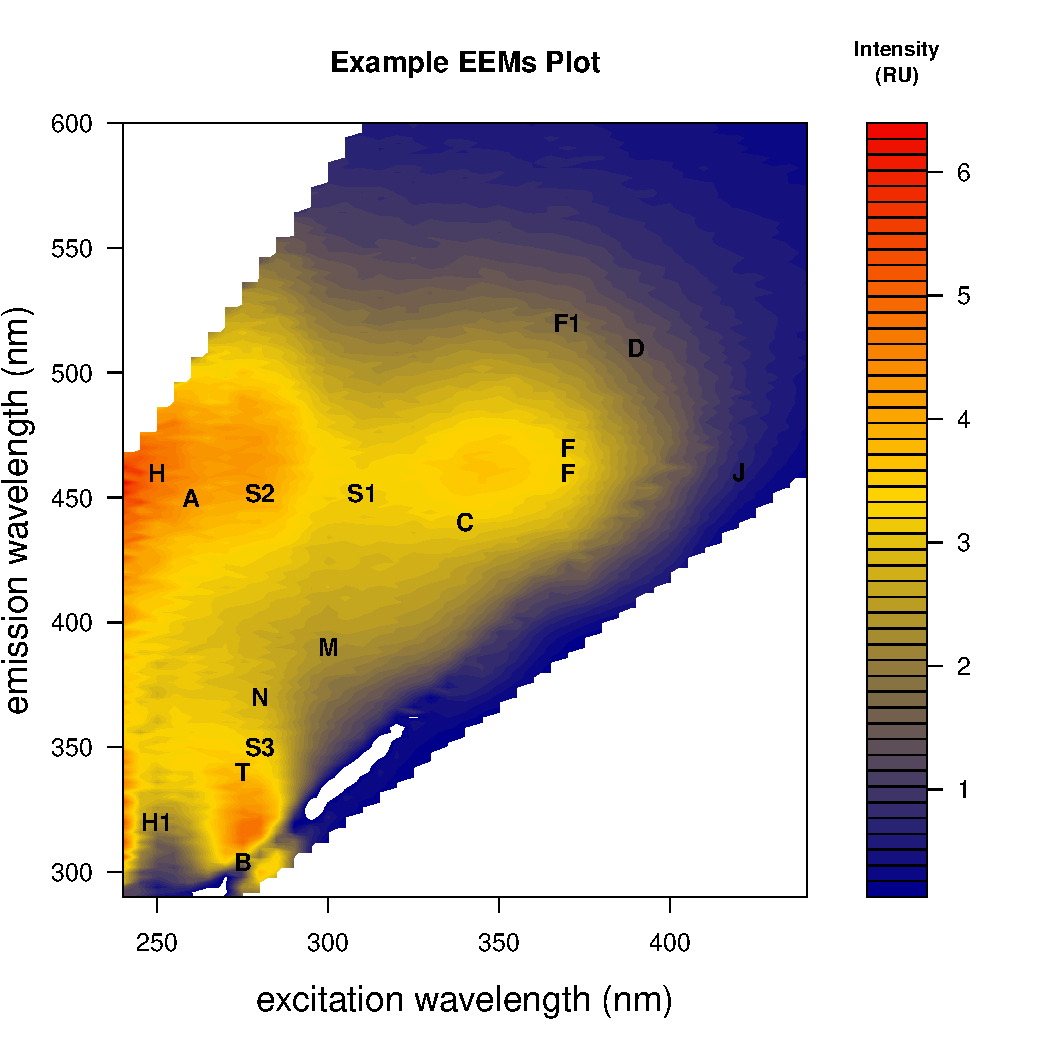
\includegraphics[width=\maxwidth]{figure/unnamed-chunk-3} 
\begin{kframe}\begin{verbatim}
NULL
\end{verbatim}
\end{kframe}
\end{knitrout}

%------------------------------------------------------------
\section{Dataframe Formatting for USGS HydroOpt}
%------------------------------------------------------------ 
The functions contained in USGSHydroOpt operate on dataframes with defined structures. Users interested in using USGSHydroOpt should format dataframes according to the structures defined in this section.

%------------------------------------------------------------
\subsection{Absorbance Data}
%------------------------------------------------------------
Absorbance data used by functions in USGSHydroOpt should be formatted such that each sample occupies a column, and one column contains the wavelength for which the absorbance measurement was measured (\emph{See example below}). The column with the wavelengths does not need to be called "wavelengths," as it is named in the example dataframe below. Since this package was developed primarily for USGS activities, the default for naming samples is "gr" then the sample number. This convention was started by the USGS California Water Sciences Center (CA WSC) and the USGS Wisconsin Water Science Center (WI WSC) follows the same naming convention to ensure standardization.

\begin{knitrout}
\definecolor{shadecolor}{rgb}{0.969, 0.969, 0.969}\color{fgcolor}\begin{kframe}
\begin{verbatim}
     gr13307    gr13351    gr13353    gr13357 wavelengths
1  0.0001296 -0.0003505 -0.0003480 -0.0002695         750
2 -0.0002367  0.0000305 -0.0000915 -0.0001407         749
3 -0.0001582 -0.0004900 -0.0006325 -0.0001534         748
4 -0.0004642 -0.0000105 -0.0000932 -0.0000245         747
5 -0.0002551 -0.0000653  0.0000841 -0.0001615         746
6 -0.0001842 -0.0002135  0.0002082  0.0001429         745
\end{verbatim}
\end{kframe}
\end{knitrout}

%------------------------------------------------------------
\subsection{Fluoresence Data}
%------------------------------------------------------------
Fluoresence data used by functions in USGSHydroOpt should also be formatted such that each sample occupies a column, and one column contains the excitation emission wavelength pairs for which the fluoresence measurment was measured (\emph{See example below}). The column with the excitation emission pairs does not need to be called "Wavelength.Pairs," as it is in the example dataframe below. Again since this package was developed for USGS activities, the default sample naming convention is "gr" followed by the sample number.

\begin{knitrout}
\definecolor{shadecolor}{rgb}{0.969, 0.969, 0.969}\color{fgcolor}\begin{kframe}
\begin{verbatim}
  Wavelength.Pairs gr13307 gr13308  gr13351  gr13352
1          240/290 0.09457 0.05358 -0.07268 -0.19368
2          240/292 0.07386 0.09194  0.45433  0.39722
3          240/294 0.08116 0.09930  0.49135  0.37943
4          240/296 0.12013 0.09138 -0.12248  0.09239
5          240/298 0.15264 0.15428  0.54694  0.14980
6          240/300 0.16467 0.13010  0.43319  0.33064
\end{verbatim}
\end{kframe}
\end{knitrout}

%------------------------------------------------------------
\subsection{Spectral Slopes Data}
%------------------------------------------------------------
Information on the upper and lower wavelength for which a spectral slope should be calculated needs to be stored in a dataframe if USGSHydroOpt is used. The dataframe should contain exactly three columns. The first column should contain the upper wavelength, the second column should contain the lower wavelength, and the third column should contain the name of the spectral slope being calculated (\emph{See example below}). The columns need to be in this exact order, although the names of the columns may be different. The data types for each column are integer, integer, and character, respectively. More spectral slopes can be added to the table than specified in the example dataframe below.

\begin{knitrout}
\definecolor{shadecolor}{rgb}{0.969, 0.969, 0.969}\color{fgcolor}\begin{kframe}
\begin{verbatim}
  wvlngth1 wvlngth2       Name
1      275      290 Sag275_295
2      290      350 Sag290_350
3      350      400 Sag350_400
4      412      676 Sag412_676
\end{verbatim}
\end{kframe}
\end{knitrout}

%------------------------------------------------------------
\subsection{Optical Summary Data}
%------------------------------------------------------------
This is the dataframe that contains many of the summary optical variables that can be produced using functions in USGSHydroOpt (\emph{See example below}). The functions in USGSHydroOpt calculate summary optical variables and add to a dataframe formatted according to the example below.  The example dataframe below is how the WI WSC stores optical summary variables. Note that this dataframe can contain other columns with metadata, for example, the sample data and time, the sample ID, or whether or not the sample went through QA/QC.

\begin{knitrout}
\definecolor{shadecolor}{rgb}{0.969, 0.969, 0.969}\color{fgcolor}\begin{kframe}
\begin{verbatim}
  GRnumber         B      T      A       J FI_2005    A254
1  gr13307  0.050997 0.1826 0.4553 0.03705   1.639 0.05228
2  gr13351 -0.245602 0.4085 3.0783 0.19110   1.456 0.43531
3  gr13353 -0.175220 0.7794 6.8624 0.56309   1.523 0.68274
4  gr13357  0.111561 0.2691 0.9451 0.06969   1.572 0.08698
5  gr13360 -0.001569 0.4593 2.8254 0.37231   1.563 0.28605
6  gr13363  0.052137 0.4892 1.9518 0.19098   1.583 0.19283
\end{verbatim}
\end{kframe}
\end{knitrout}

However, also note that summary optical variable names in the dataframe must be identical to those specified in the table below. 

\begin{knitrout}
\definecolor{shadecolor}{rgb}{0.969, 0.969, 0.969}\color{fgcolor}\begin{kframe}


{\ttfamily\noindent\bfseries\color{errorcolor}{Error: object 'summaryOpticalVars' not found}}

{\ttfamily\noindent\bfseries\color{errorcolor}{Error: object 'summaryOpticalVars' not found}}\end{kframe}
\end{knitrout}





\end{document}
